\usetikzlibrary{arrows.meta,calc}
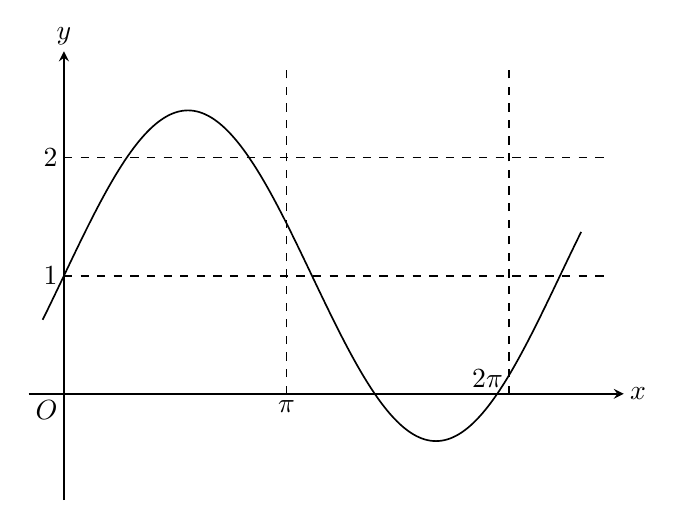
\begin{tikzpicture}[x=0.9cm,y=1.5cm,line width=.6pt,>=stealth,font=\normalsize]
\draw[->] (-0.5,0) -- (7.9,0) node[right,inner sep=0pt,xshift=2pt] {$x$};
\draw[->] (0,-0.9) -- (0,2.9) node[above,inner sep=0pt,yshift=2pt] {$y$};
\node[below left,inner sep=0pt,xshift=-2pt,yshift=-2pt] at (0,0) {$O$};
\draw[dashed] (0,2) -- (7.7,2);
\draw[dashed] (0,1) -- (7.7,1);
\draw[dashed] (3.1415927,0) -- (3.1415927,2.8);
\draw[dashed] (6.2831853,0) -- (6.2831853,2.8);
\draw[domain=-0.3:7.3,samples=220] plot (\x,{1+1.4*sin(\x*360/7)});
\node[left,inner sep=0pt,xshift=-2pt] at (0,2) {$2$};
\node[left,inner sep=0pt,xshift=-2pt] at (0,1) {$1$};
\node[below,inner sep=0pt,yshift=-2pt] at (3.1415927,0) {$\pi$};
\node[above left,inner sep=0pt,xshift=-2pt,yshift=2pt] at (6.2831853,0) {$2\pi$};
\end{tikzpicture}
